In order to refer to our project management, we will talk about the toolings and methods we used,
as summarised in the figure \ref{fig:management:tooling}.

\begin{figure}
    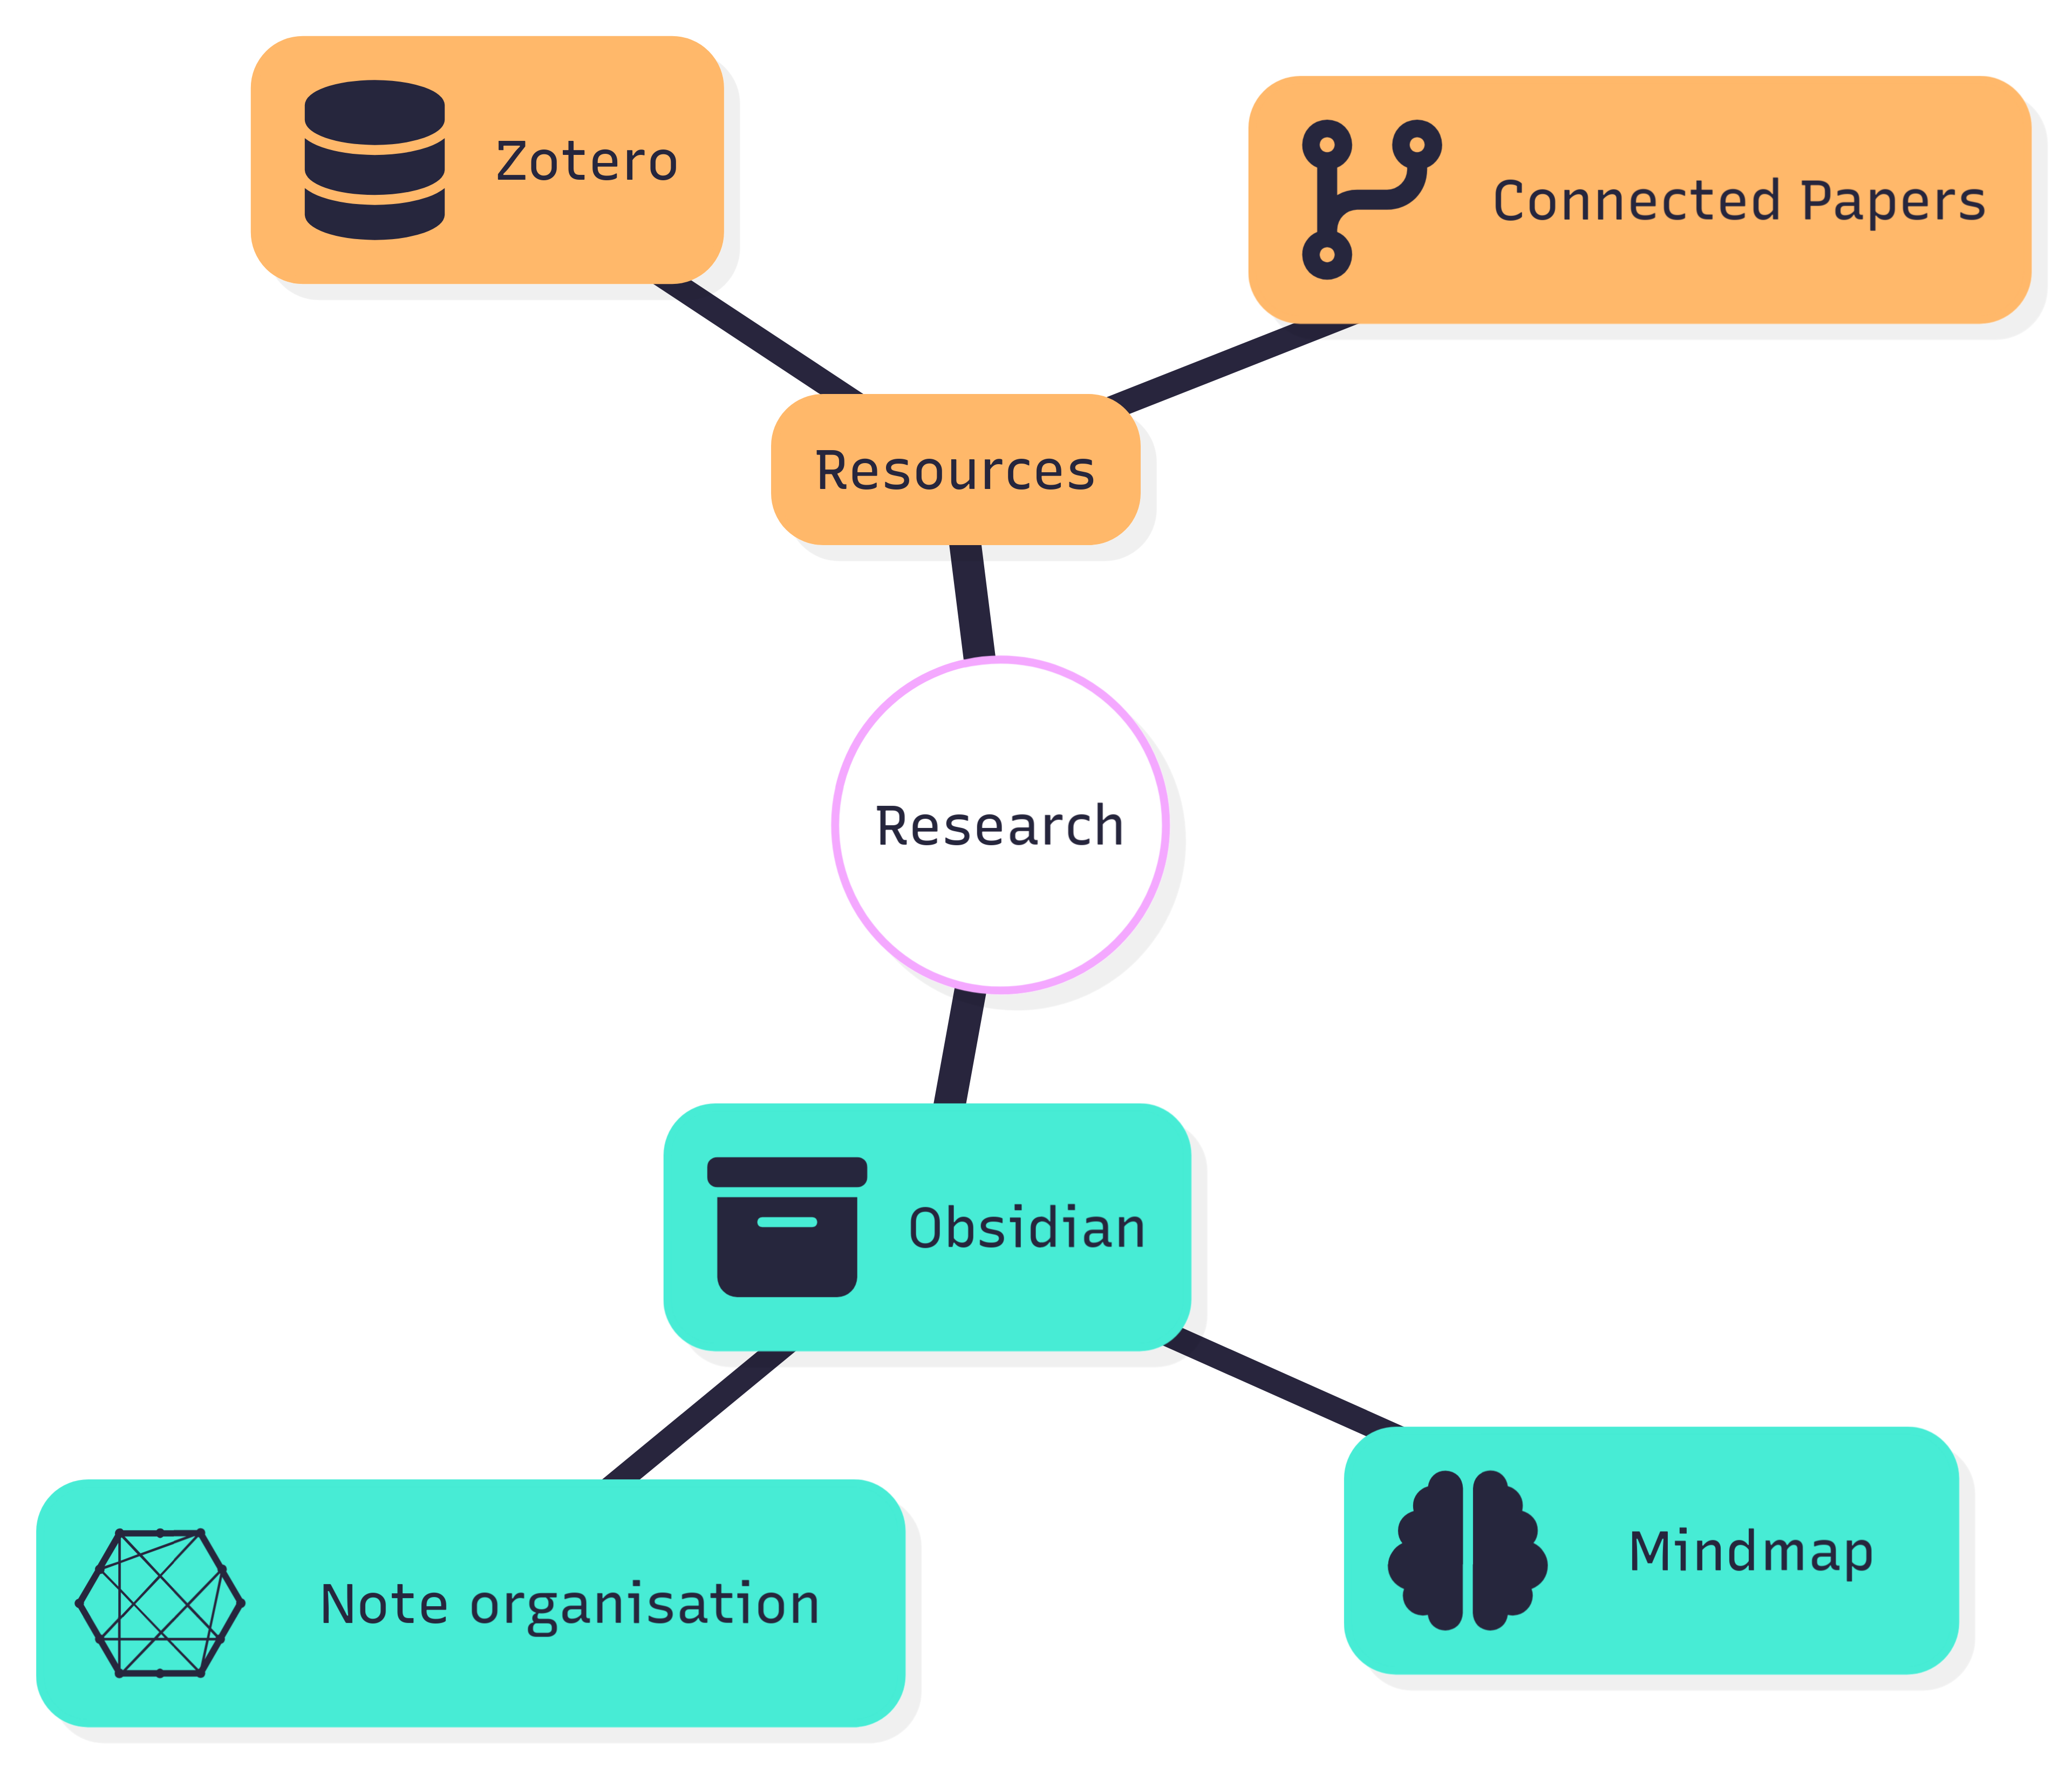
\includegraphics[width=0.45\textwidth]{assets/research-visualisation.png}
    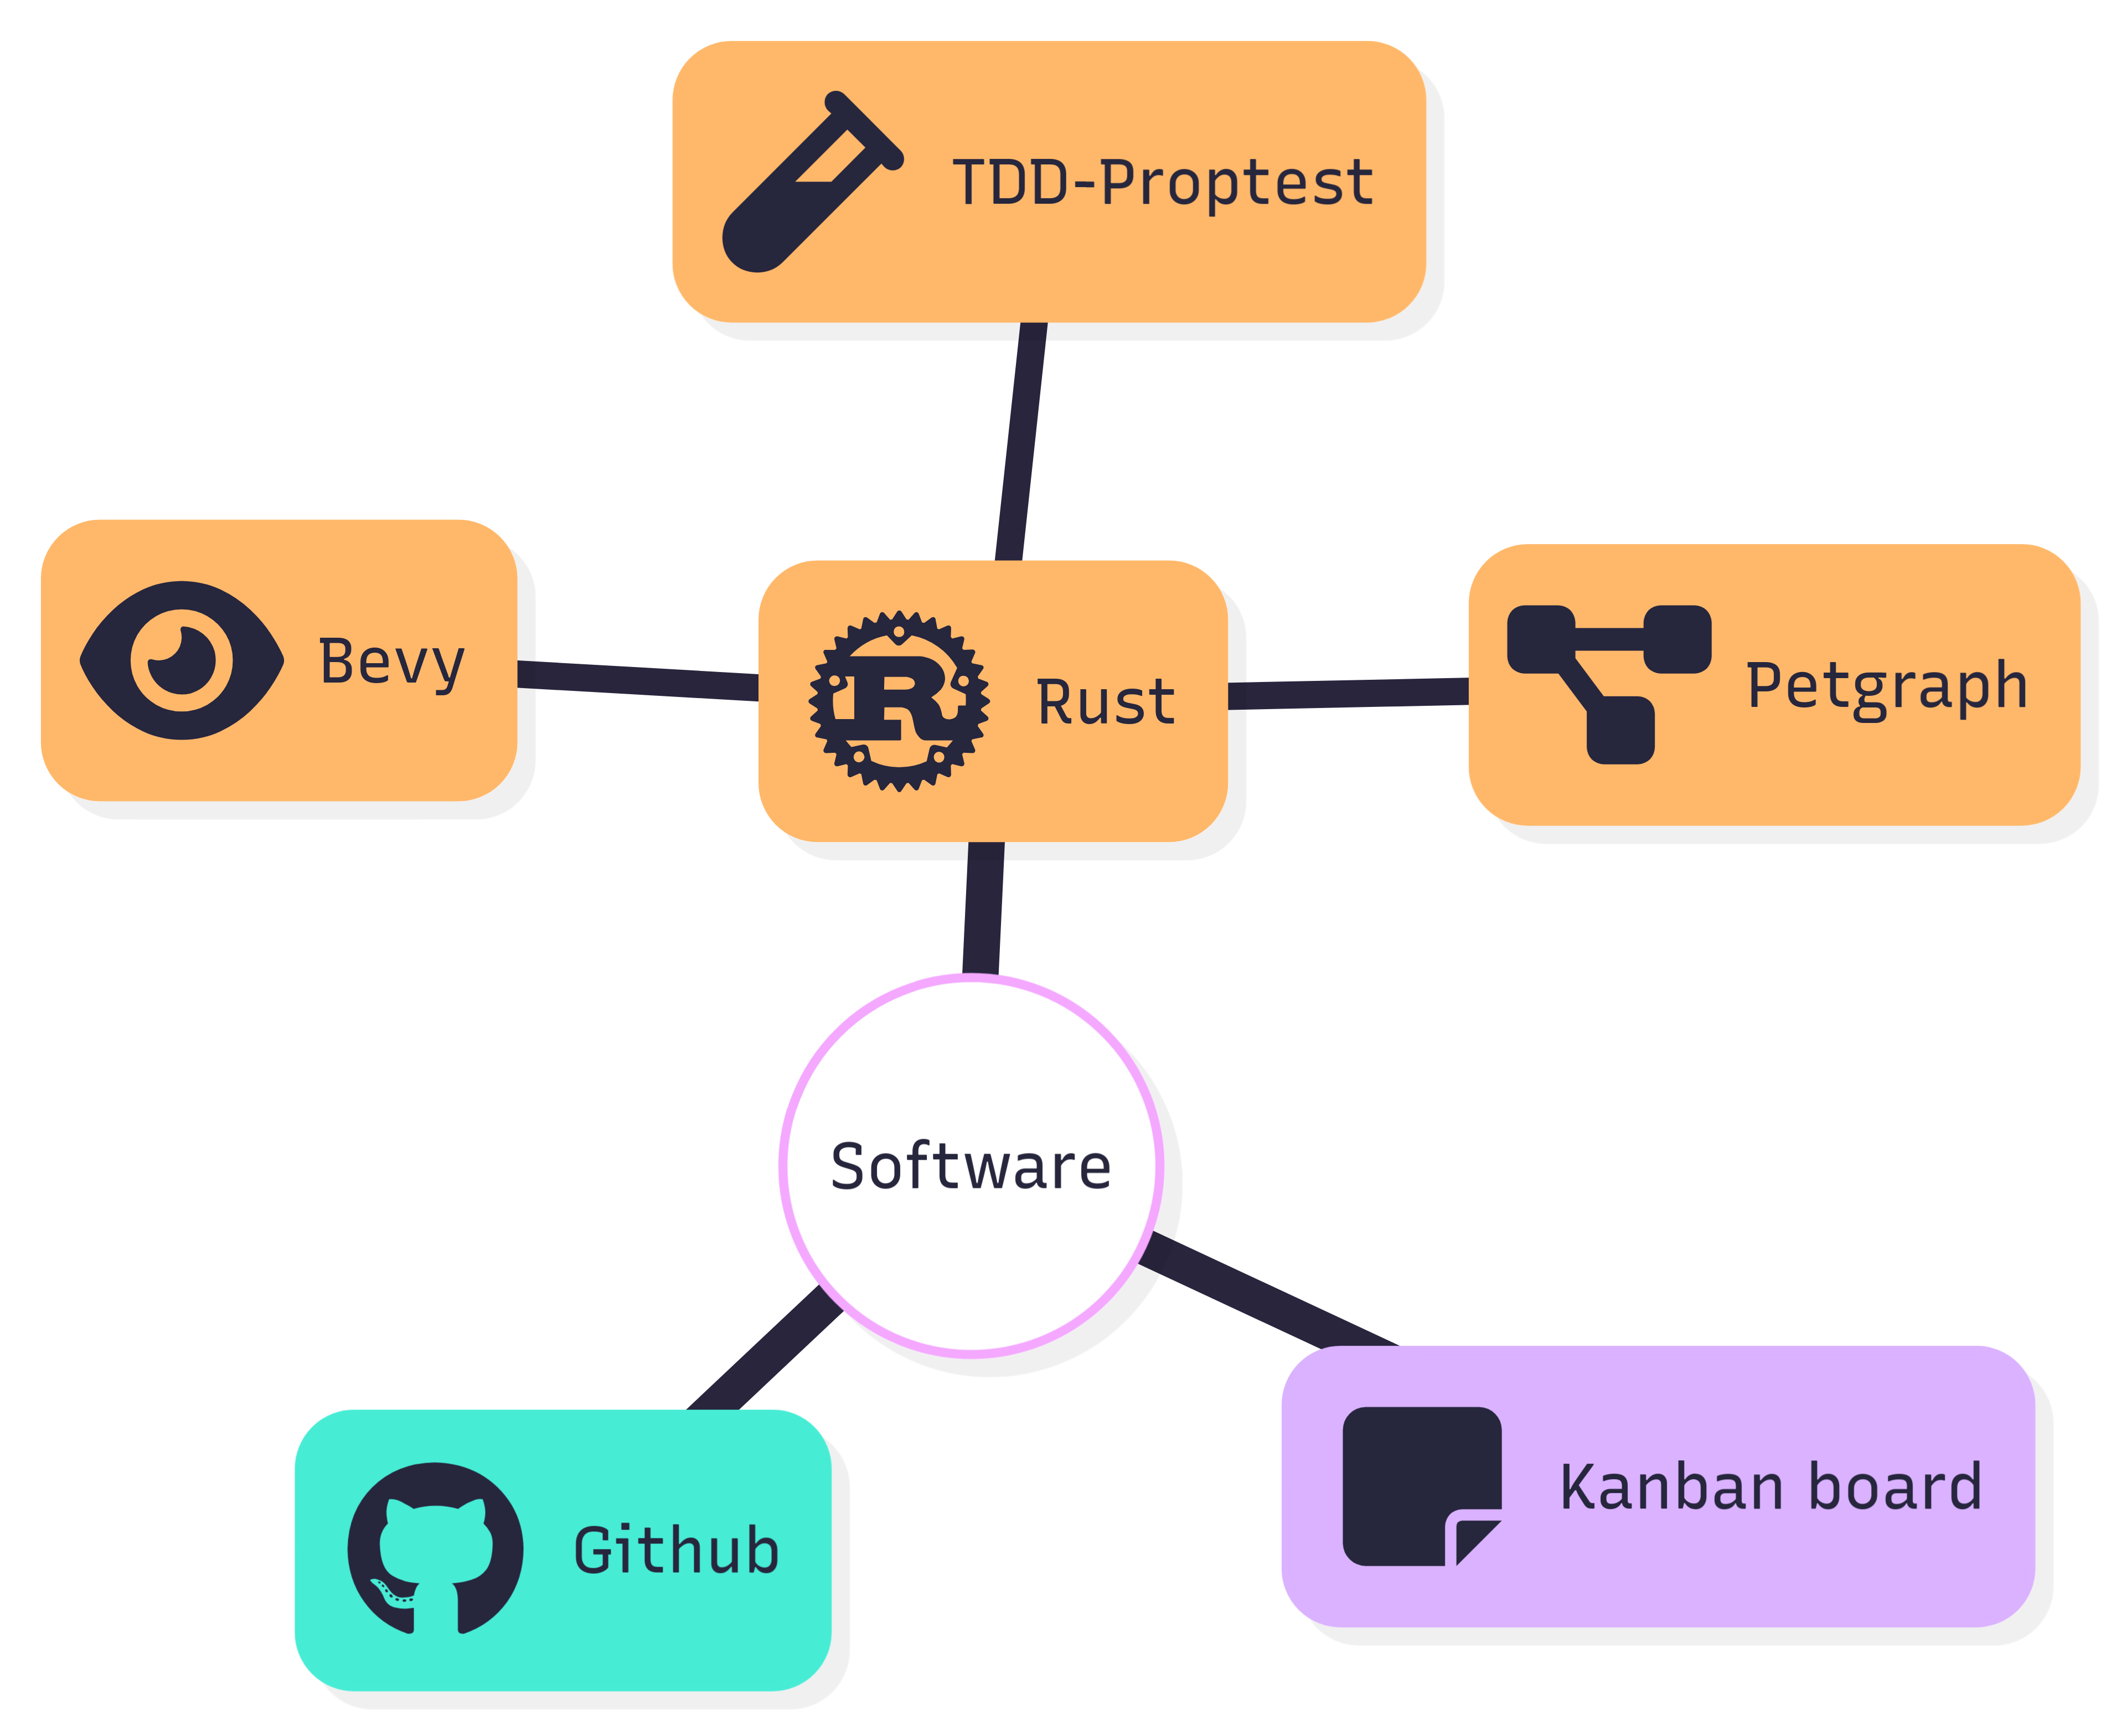
\includegraphics[width=0.45\textwidth]{assets/software-map.png}
    \caption{Tooling}\label{fig:management:tooling}
\end{figure}

Our project also includes the development of a visualisation tool for creation
and verification of several \textsc{PureCircuit} instances. We opted with \textit{Rust},
as the main language of development, due to its high and low level features.
From the one hand, \textit{Rust} can efficiently handle memory allocation safely
with its clever usage of the Borrower-Ownership framework. Conversely, it implements
a strongly typed system with help of generics, associated types and algebraic types
allowing us to create a versatile and compact library. Given the above, we utilise
techniques such as \texttt{Proptest}, where we create strategic randomized tests
that check whether  function follows an expected property. On the other hand
we make use of \texttt{Petgraph}, which is a sophisticated library that handles
graph-like structures in \textit{Rust}.


For visualisation we decided to go with \textit{Bevy}. \textit{Bevy} is a
game engine that uses the \textit{ECS} software architecture. A general
workflow of an \textit{ECS} system can be described as such: a state 
contains entities, each of which is composed of components or properties.
A system is a specialised method that gathers entities based on their components
and describes an interaction between them. This whole process can be visualised
in the figure \ref{fig:soft:ecs-workflow}


\begin{figure}[h!]
    \centering
    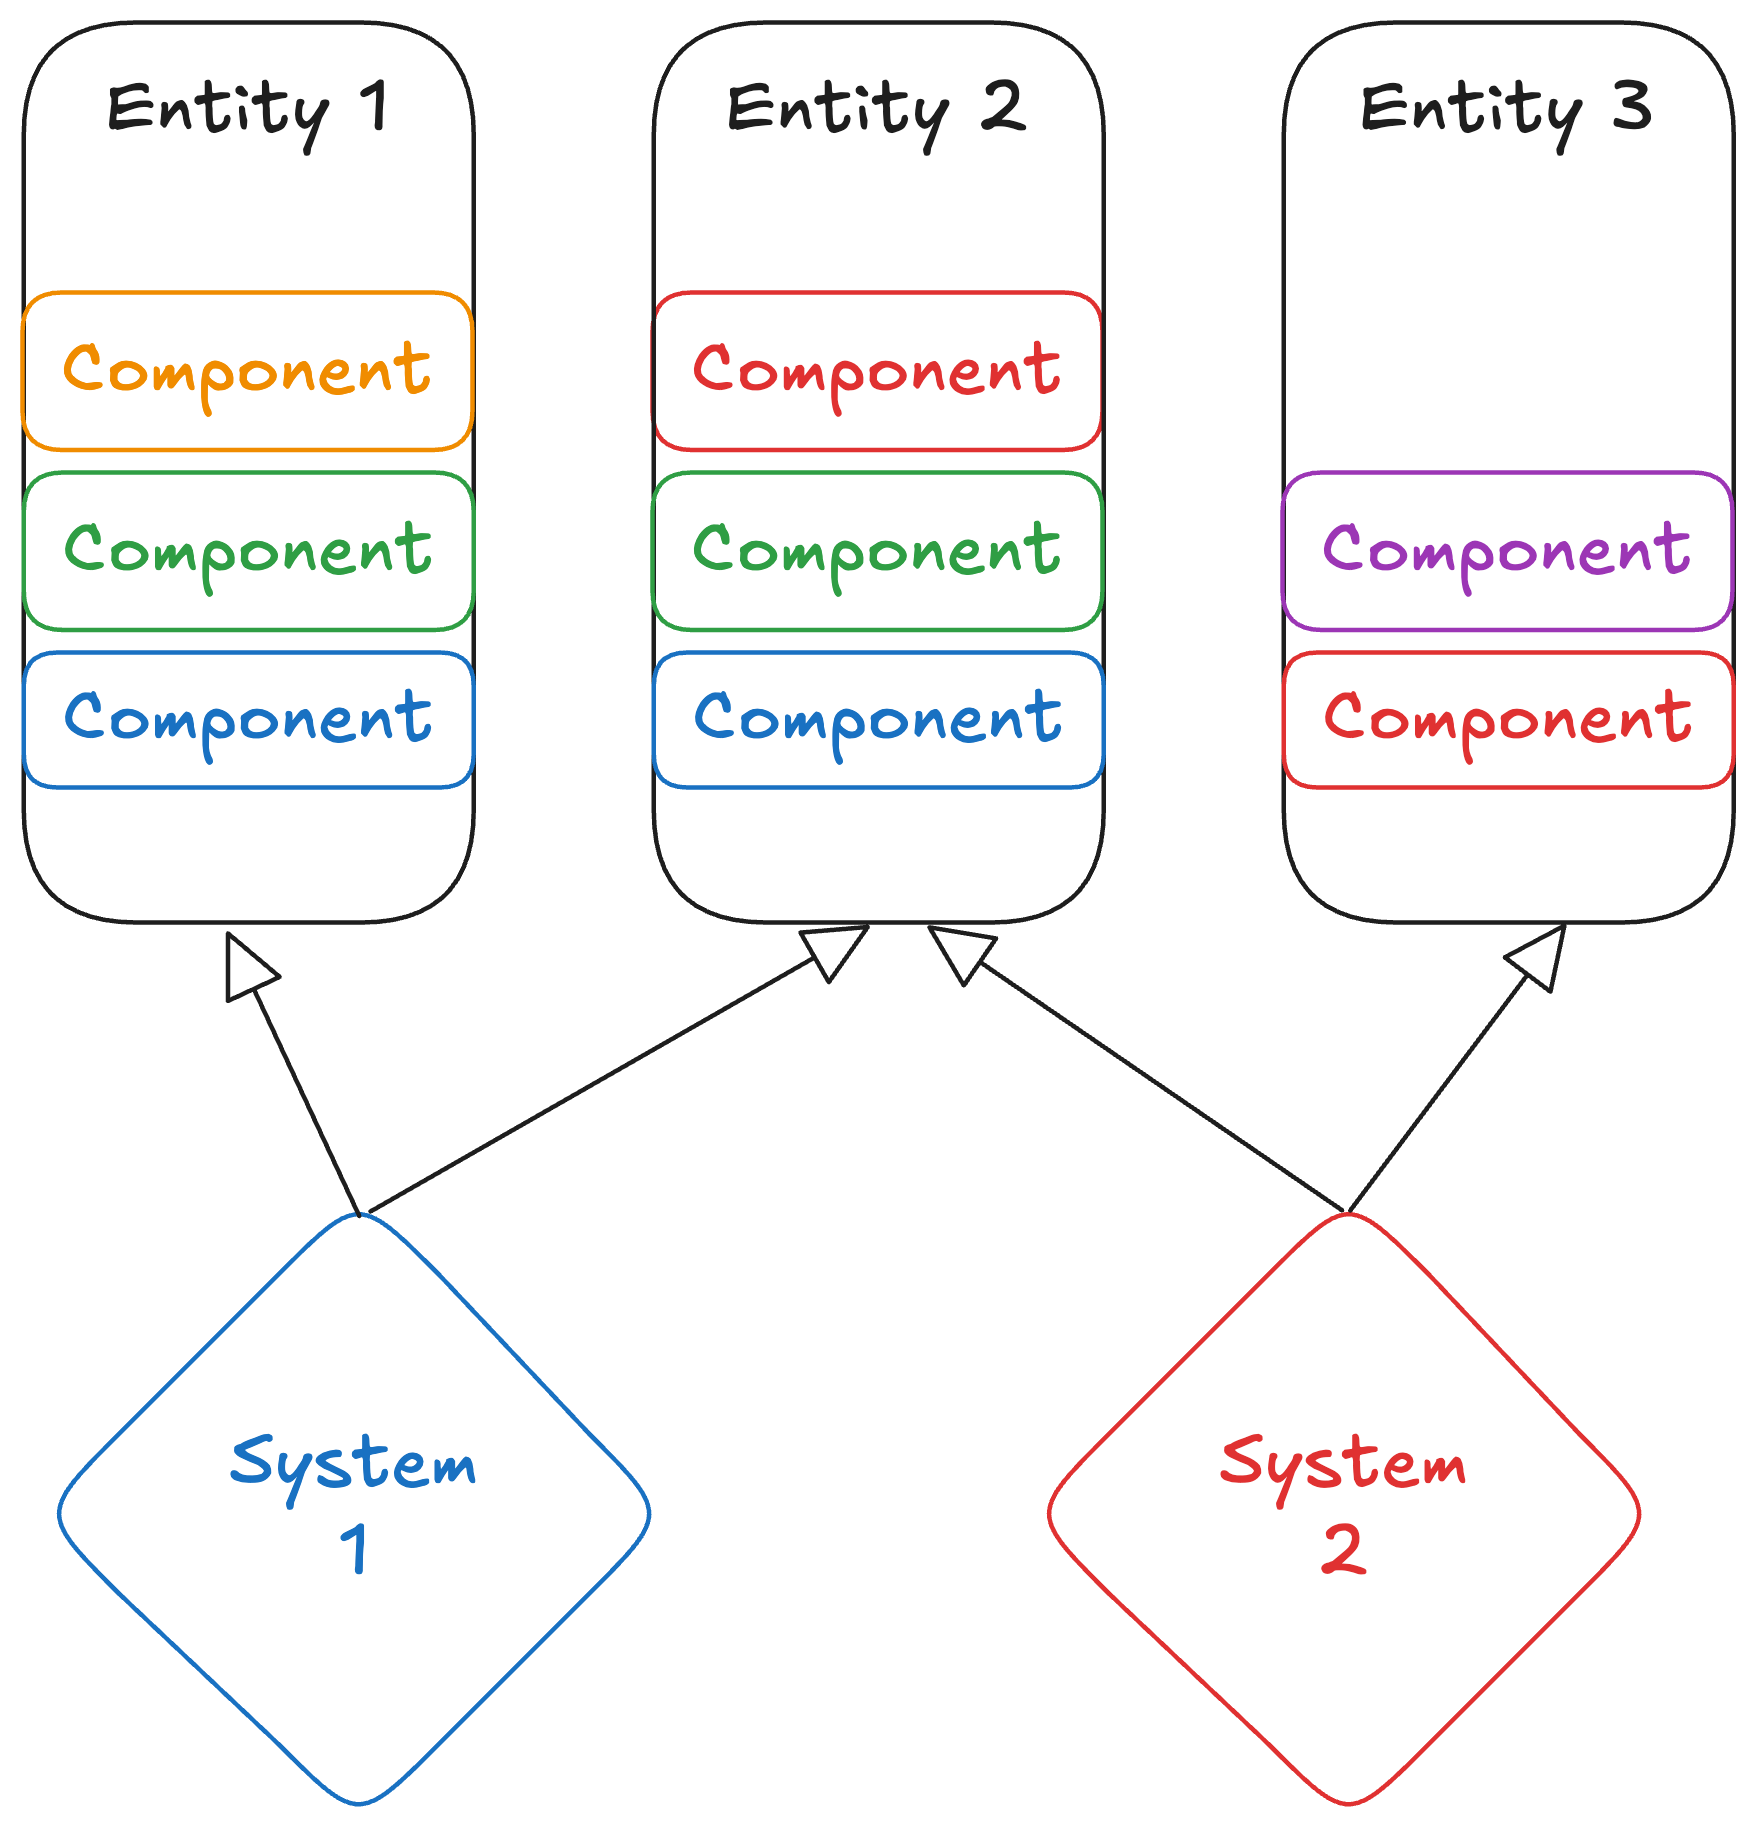
\includegraphics[width=0.35\textwidth]{assets/ECS-visualisatoin.png}
    \caption{ECS workflow visualisation}
    \label{fig:soft:ecs-workflow}
\end{figure}

With regards to the our research management, our core tool came
through the usage of obsidian. As we can see in the figure \ref{fig:management:tooling}, 
\texttt{Obsidian} beyond its traditional usage of note taking, it comes
with several handy tools such as note organisation and mind-mapping.
These can be seen in the figure \ref{fig:theory:obsidian-usages}, where we utilised connections across notes as well as
its drawings or other thought organisation tools in order
experiment and manage ideas.



\begin{figure}[h!]
    \centering
    \subfloat[Obsidian Graph]{
        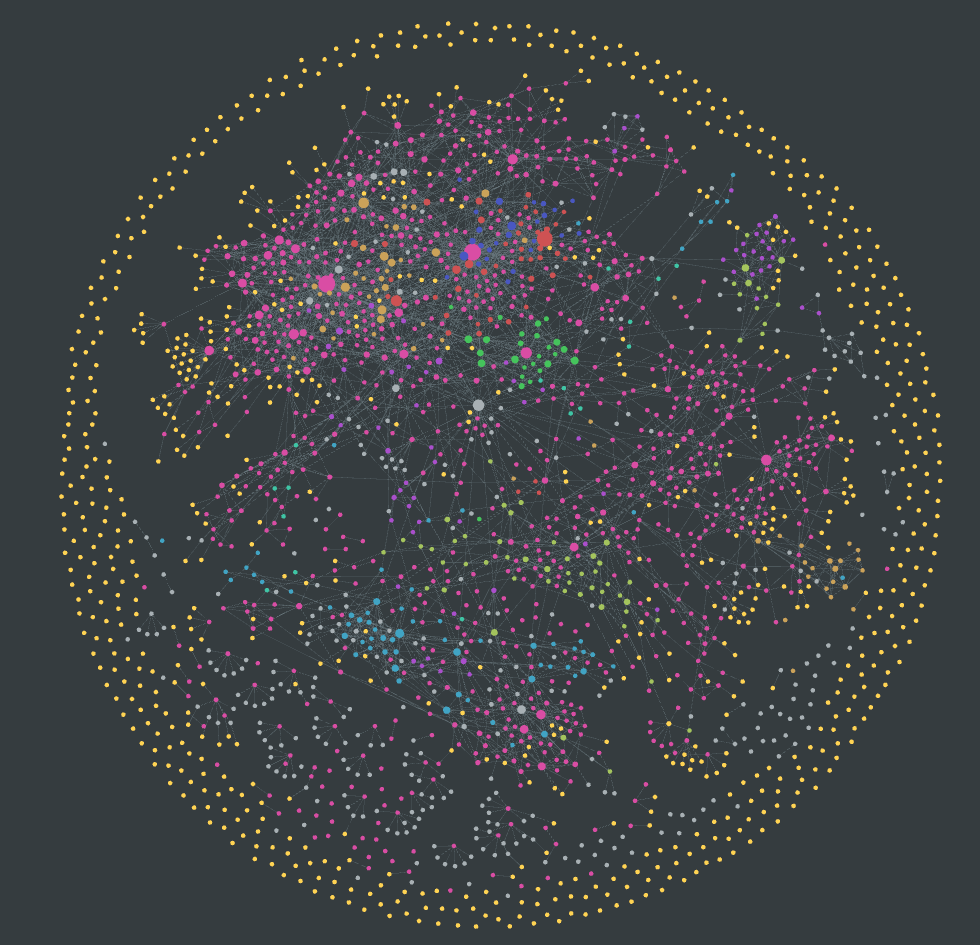
\includegraphics[width=0.3\linewidth]{assets/obsidian_graph.png}
        \label{fig:theory:obsidian-graph}
    }
    \subfloat[Obsidian Canvas]{
        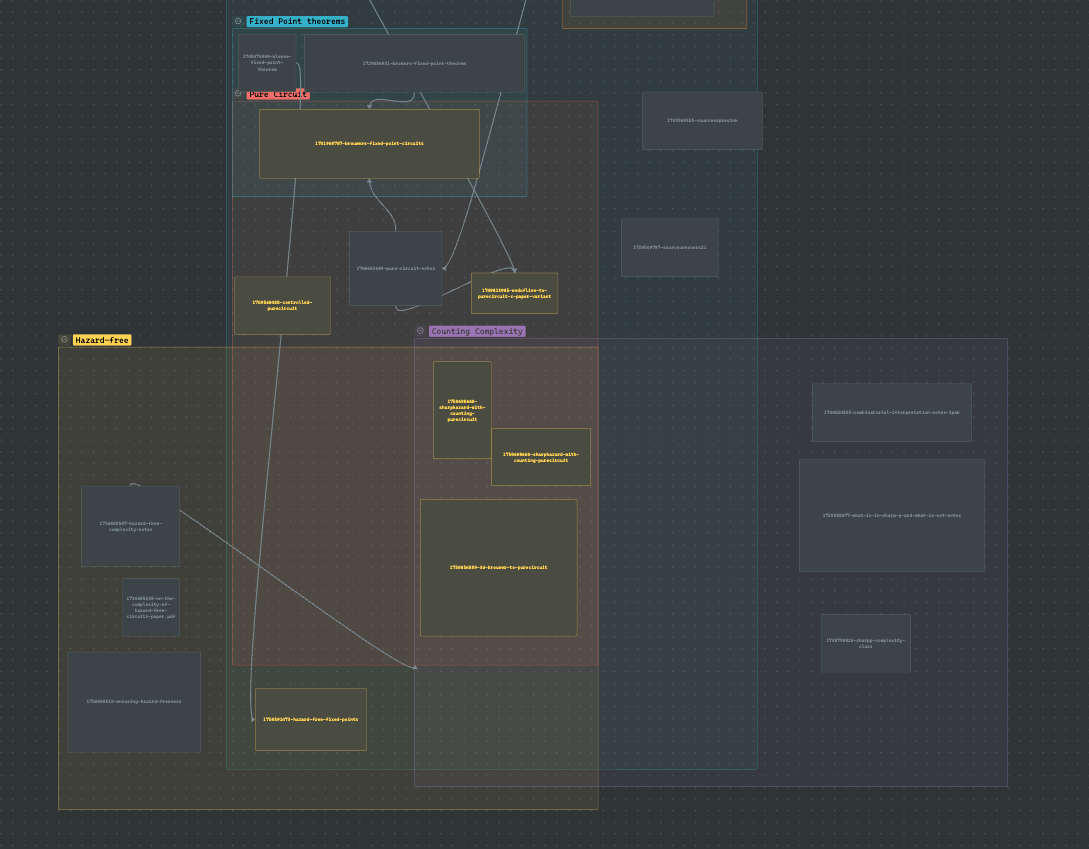
\includegraphics[width=0.3\linewidth]{assets/obsidian-canvas.png}
        \label{fig:theory:obsidian-canvas}
    }
    \subfloat[Obsidian mindmap]{
        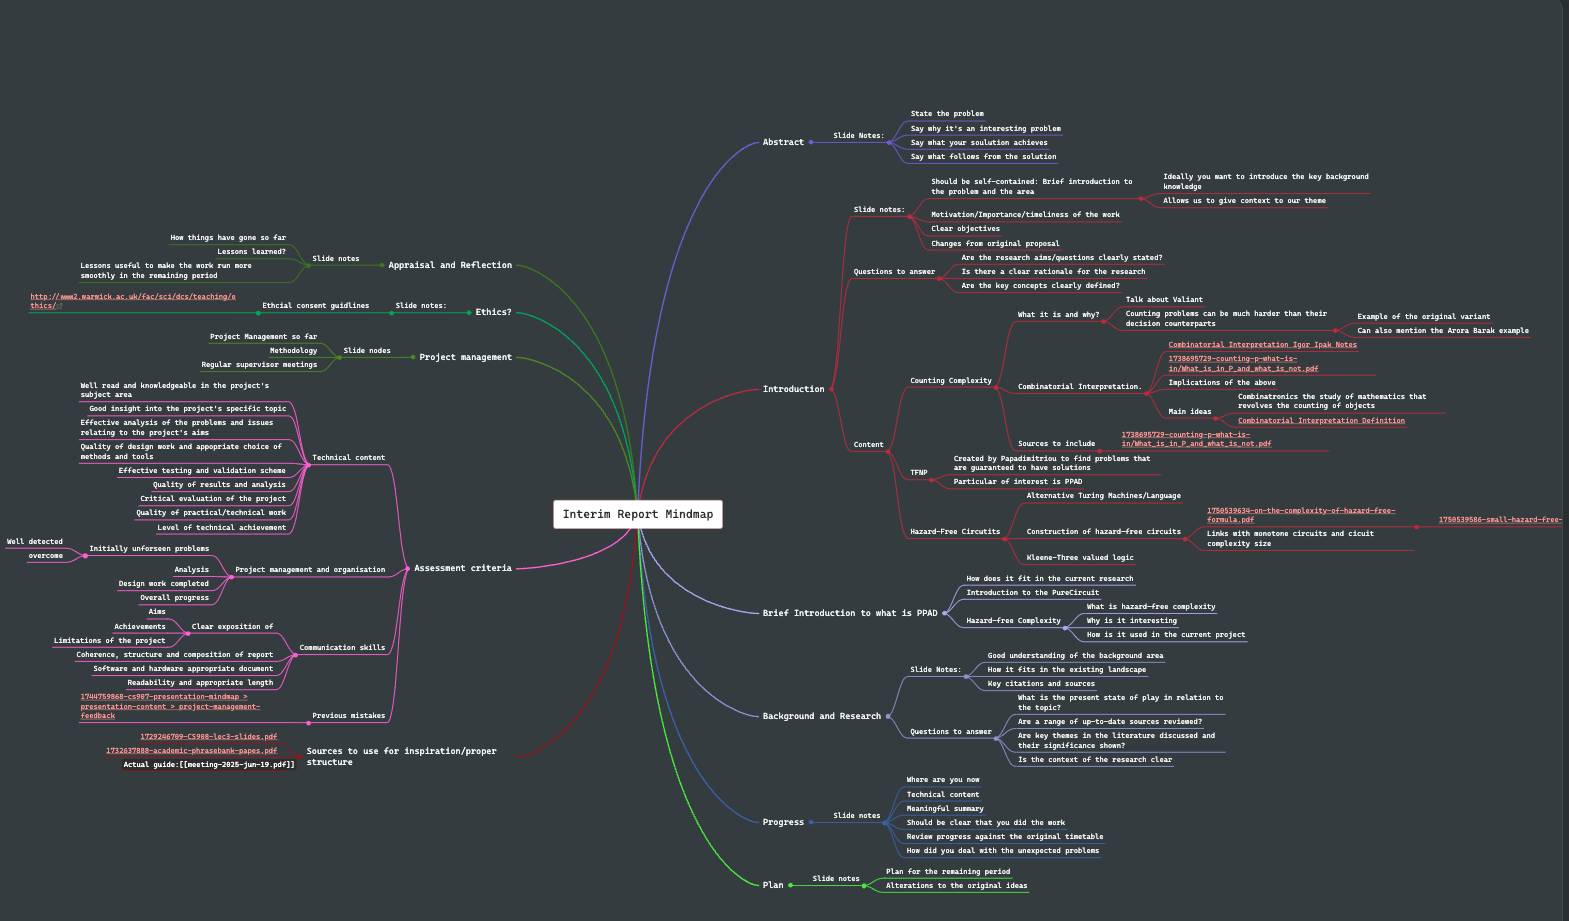
\includegraphics[width=0.3\linewidth]{assets/obsidian_mindmap.png}
        \label{fig:theory:obsidian-mindmap}
    }
    \caption{Usages of Obsidian}
    \label{fig:theory:obsidian-usages}
\end{figure}



\subsection{Risk Management}

With regards to risks and mitigations, the biggest risk we face
is the inability to resolve our main question. Due to the
limited literature surrounding \textsc{PureCircuit} and its
counting nature as well as the recency in the development of
$\textsc{TFNP} -1$, our question could go into many directions.
The discovery of our reduction allowed us to step closer to our question
and in our table \ref{tab:management:risk-management}, we will analyze this is greater depth.
The general mitigation strategy we can do is to keep researching, keep
finding connections until we can connect all the necessary pieces to do the jump.

\begin{table}[h!]
    \centering
    \begin{tabularx}{0.95\textwidth}{|Y|Y|Y|Y|Y|}
            \hline
            \textbf{Severity} & \textbf{Probability} & \textbf{Mitigation} & \textbf{Mitigation} & \textbf{Address} \\
            \hhline{|=|=|=|=|=|}
            High   & Medium & Software may not be feasible within the remaining time frame. & Focus on the the first objective where the project. Restrict to solution finding or counting when the number of nodes is small. & Not yet      \\ \hline
            Low    & Medium & Software not identifying a correct solution & Usage of TDD techniques and property testing to ensure correctness.  Comparison with hand-made instances & Not yet      \\ \hline
            High   & High   & Inability to extend the reductions of the PureCircuit problem to SourceOrExcess & Find a path of parsimonious reductions between the two problems. If we cannot ensure a one-to-one relation between the solutions, we will focus on $1-c$ for some $c \in \mathbb{N}$  & $\checkmark$ \\ \hline
            Medium & High   & Inability to prove the main conjecture & We can make some heuristical arguments or find reductions between other problems. We argue that if we are able to unravel enough correlations, we will hope to at least bridge the problems. Develop useful gadgets one can use with PureCircuit & Not yet     \\ \hline
            High   & High   & Incorrect proofs or reductions. & Analyse the problem under different constraints. Apply the duck method, where attempt to explain the solution to a person which not necesserily an expert. Validate proof with supervisor & Not yet  \\ \hline
            High   & Medium & Develop combinatorial friendly variants of \textsc{PureCircuit} & Apply robustness on the gate set of \textsc{PureCircuit}. Develop new gates or variants are easier to work with.  & $\checkmark$  \\ \hline
    \end{tabularx}
    \caption{Risk managment table.}
    \label{tab:management:risk-management}
\end{table}
\FloatBarrier


From our table, it is worth expanding on some of the points. The best method
we found when tackling this problem is when we try to uncover reductions between other
PPAD problems or when trying to incorporate gadgets from Kleene theory. We hope
that by expereminting enough we will be able to get close to resolve our conjectures.
In addition, for the last point, we made several efforts to ensure our problem is
\textsc{PPAD}-complete and combinatorial friendly, by trying to restrict the \textsc{Purify} gate. 
We soon realised that any methods that detect the $\bot$ value or try to eliminate ultimately
fail. The observation can be based on a continuity argument that Marino created
\cite{marino_GeneralTheoryMetastable_1981} and in general any possible extensions or gates we can
add seem to adhere continuity. (TODO)
